\documentclass{standalone}
\usepackage{tikz}

\begin{document}
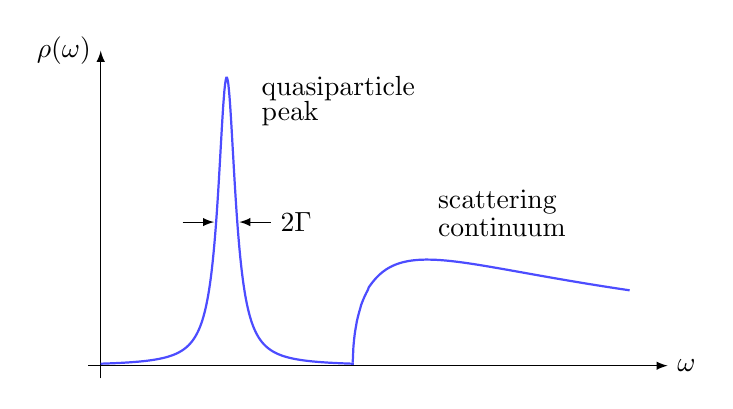
\begin{tikzpicture}[scale=1.6]
  % Draw axes
  \draw[-latex] (-0.1,0) -- (4.5,0) node[right] {$\omega$};
  \draw[-latex] (0,-0.1) -- (0,2.5) node[left] {$\rho(\omega)$};
  
  \draw[domain=0:2.0138, samples=400, variable=\x, blue!70, thick] plot (\x, {0.016/((\x-1)^2+0.007)});
  \draw[domain=2.00016:4.2, samples=400, variable=\x, blue!70, thick] plot (\x, {8*(\x-2)^(1/2)/(\x^2+(\x-2))});
  
  \draw[-latex] (0.65,1.14) -- (0.9,1.14) node[right] {};
  \draw[latex-] (1.1,1.14) -- (1.35,1.14) node[right] {$2\Gamma$};
  
  \draw (2.6,1.3) node[right] {scattering};
  \draw (2.6,1.1) node[right] {continuum};
  \draw (1.2,2.2) node[right] {quasiparticle};
  \draw (1.2,2.0) node[right] {peak};

\end{tikzpicture}
\end{document}